\chapter{Lux.jl: Bridging Scientific Computing and Deep Learning}
\label{chapter:lux_bridging_scientific_computing_and_deep_learning}

% \citet{Rackauckas2020GeneralizedPL}

\section{Design Philosophy}
\label{sec:design_philosophy}

\section{Scientific Computing vs Deep Learning}
\label{sec:scientific_computing_vs_deep_learning}

\section{Composability via Generic Parameterization}
\label{sec:composability}

\todo{texts for what the code is doing}

\subsection{Neural Differential Equations}
\label{subsec:differential_equations_lux}

\todo{show how to use lux to solve differential equations}

\subsection{Differentiable Convex Optimization}
\label{subsec:convex_optimization_lux}

\todo{combine lux with jump.jl}

\subsection{Gradient Free Optimization Algorithms}
\label{subsec:evolutionary_alg_lux}

Lux allows the parameters of a complicated neural network to be represented as a flattened vector. This allows it to interface directly with optimization packages without any glue code. In this example, we will train a neural network with gradient-free optimization algorithms to learn the function:
%
\begin{align}
  r(\theta) &= e^{sin(\theta)} - 2cos(4\theta) + sin\left(\frac{2\theta - \pi}{12}\right)^5\\
  \texttt{where } \theta &\in [0, 2\pi]
\end{align}
%
We will use algorithms implemented in packages that are agnostic to the specifics of Lux:
%
\begin{itemize}
  \item Covariance Matrix Adaptation Evolutionary Strategy (CMAES) \tocite from CMAEvolutionStrategy.jl \tocite.
  \item LN\_COBYLA \tocite from NLopt.jl \tocite \todo{highlight that it is a C library underneath}.
\end{itemize}
%

\todo{Showcased CMAES, add other algorithms and show how easy it is to add new algorithms}

\inputminted[linenos, breaklines, fontsize=\scriptsize]{julia}{../code/gfopt.jl}

\begin{figure}[t]
  \centering
  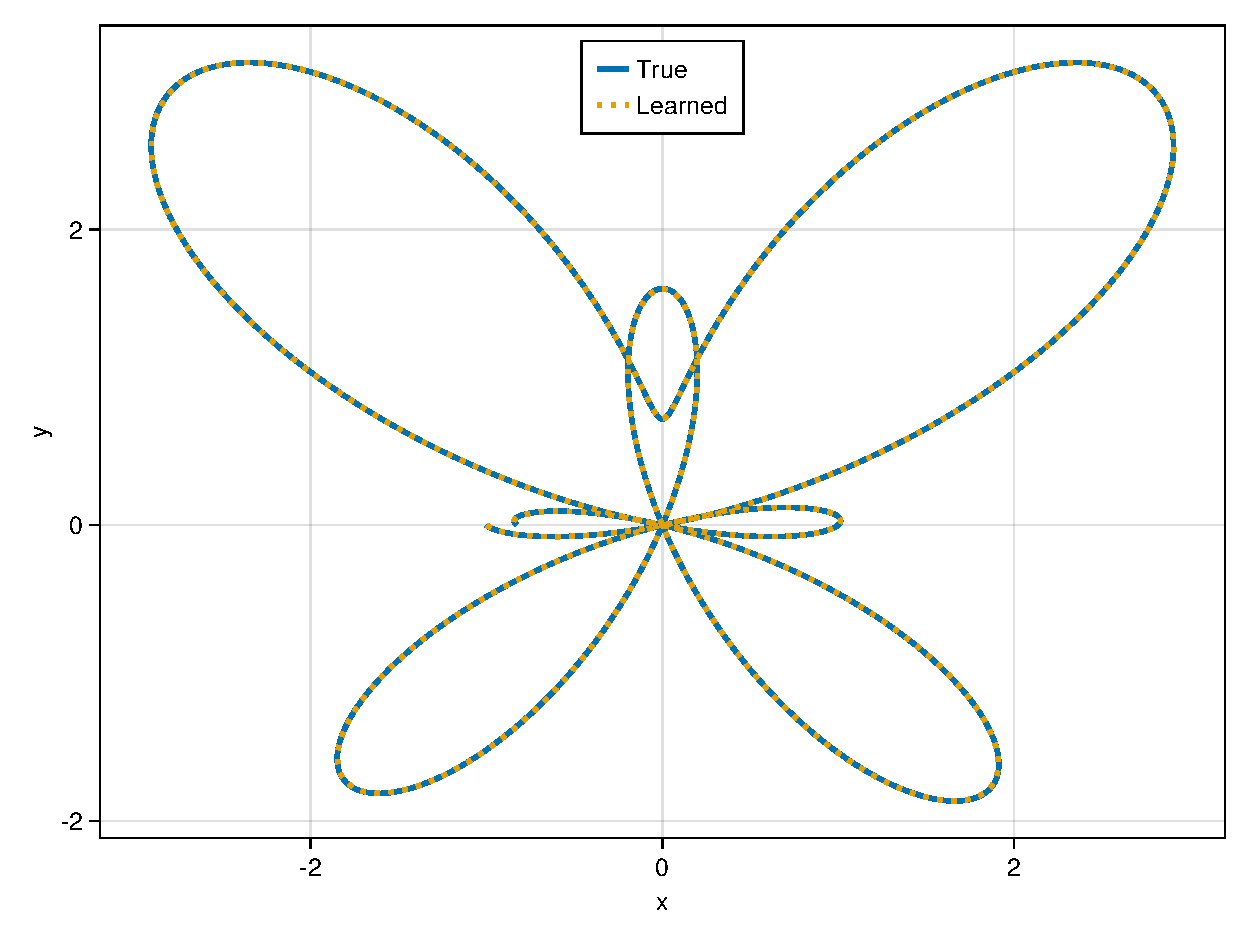
\includegraphics[width=0.8\textwidth]{../figures/lux/cmaes_plot.pdf}
  \caption{CMA-ES optimization to learn the parameters of a neural network that approximates the function $r(\theta) = e^{sin(\theta)} - 2cos(4\theta) + sin\left(\frac{2\theta - \pi}{12}\right)^5$.}
  \label{fig:lux_cmaes_plot}
\end{figure}

\subsection{Physics Informed Neural Networks}
\label{subsec:physics_informed_neural_networks_lux}

\todo{I want to showcase higher-order AD: not sure what example to use}

In this section, we will describe how to model Physics-Informed Neural Networks (PINNs)~\citep{raissi2019physics} that leverage neural networks to solve Partial Differential Equations~(PDEs). 

% \inputminted[linenos, fontsize=\footnotesize]{julia}{../code/pinn.jl}

NeuralPDEs.jl~\citep{zubov2021neuralpde} extends Lux.jl to provide neural networks solvers for PDEs using PINNs.

% \subsection{Higher Order Taylor Mode Automatic Differentiation}
% \label{subsec:higher_order_taylor_mode_automatic_differentiation}

\section{Leveraging Cross-Language Capabilities}
\label{sec:cross_language_capabilities}

\todo{pycallchainrules for lux + pytorch and lux + jax}

\section{Performance}
\label{sec:performance_lux}

\todo{compare against flux and maybe knet}

\section{Discussion}
\label{sec:discussion_lux}

\subsection{Current Limitations}
\label{subsec:current_limitations}
